% generated by Docutils <http://docutils.sourceforge.net/>
\documentclass[a4paper,english]{article}
\usepackage{fixltx2e} % LaTeX patches, \textsubscript
\usepackage{cmap} % fix search and cut-and-paste in PDF
\usepackage{babel}
\usepackage{mathpazo}
\usepackage{setspace}
\usepackage{mathabx}
\usepackage[T1]{fontenc}
\usepackage[utf8]{inputenc}
\usepackage{ifthen}
\usepackage{float} % float configuration
\floatplacement{figure}{H} % place figures here definitely
\usepackage{graphicx}

\usepackage[colorlinks=true,linkcolor=blue,urlcolor=blue]{hyperref}
\hypersetup{
  pdftitle={Magic Lantern 0.2 for Canon 550D, Firmware 1.0.9 -- User's Guide},
  pdfauthor = {Alex Dumitrache <broscutamaker@gmail.com>},
  pdfpagelayout = {OneColumn},
  pdfpagemode = {UseNone},
  pdfstartview = {FitH},
  pdfborder = {0 0 0}
}
\usepackage[letterpaper, total={14.5cm, 22cm}, centering]{geometry}

\setlength{\parskip}{1.5mm plus2mm}
\setlength{\parindent}{0mm}

\let\olditemize=\itemize
\let\oldenumerate=\enumerate

\def\itemize{
\olditemize
\setlength{\itemsep}{0.5pt}
}
\def\enumerate{
\oldenumerate
\setlength{\itemsep}{0.5pt}
}

%%% Body
\begin{document}
\title{Magic Lantern 0.2 for Canon 550D, firmware 1.0.9\\User's Guide}
\author{\url{http://magiclantern.wikia.com/550D}}
\maketitle

\vspace{5mm}
\begin{center}
\setstretch{1.1}

\begin{minipage}{13cm}
\input{credits.tex}
\end{minipage}
\vspace{5mm}

\begin{minipage}{13cm}
Magic Lantern is being developed by independent film makers in our spare time and at risk to our beloved cameras. We hope that it saves you time and aggravation on set, and we'd appreciate your support. You can help by \href{https://www.paypal.com/cgi-bin/webscr?cmd=_donations&business=ELJ6U9GGFPL3U&lc=RO&item_name=Magic%20Lantern%20firmware%20for%20Canon%20550D&currency_code=EUR&bn=PP%2dDonationsBF%3abtn_donate_LG%2egif%3aNonHostedGuest}{donating via PayPal}, or through equipment donations. You can also \href{mailto:broscutamaker@gmail.com}{contact me (Alex) via email}. Thanks!

\vspace{2mm}
\hskip1mm \href{https://www.paypal.com/cgi-bin/webscr?cmd=_donations&business=ELJ6U9GGFPL3U&lc=RO&item_name=Magic%20Lantern%20firmware%20for%20Canon%20550D&currency_code=EUR&bn=PP%2dDonationsBF%3abtn_donate_LG%2egif%3aNonHostedGuest}{
\includegraphics[width=1.5cm]{donate.png}}
\end{minipage}
\end{center}


\newpage
%~ \tableofcontents
%~ \newpage


{ \setlength{\parskip}{0.5mm}

%___________________________________________________________________________

\section*{Features%
  \phantomsection%
  %
  \label{features}%
}
%
\begin{itemize}

\item Audio: \hyperref[disable-agc]{disable AGC} and digital filters, \hyperref[audio-meters]{audio meters}, \hyperref[manual-audio-controls]{manual audio controls}, selectable \hyperref[input-source]{input source} (internal, internal+external, external stereo, \hyperref[balanced]{balanced}), \hyperref[audio-monitoring]{audio monitoring} via USB.

\item Exposure helpers: \hyperref[zebras]{zebras}, \hyperref[false-color]{false color}, \hyperref[histogram]{histogram}, \hyperref[waveform]{waveform}, \hyperref[spotmeter]{spotmeter}.

\item Focus tools: \hyperref[focus-peaking]{focus peaking}, \hyperref[focus-graph]{focus graph}, \hyperref[trap-focus]{trap focus}, \hyperref[rack-focus]{rack focus}, \hyperref[focus-stacking]{focus stacking}, \hyperref[zoom-in-face-detect-mode]{zoom in Face Detect mode}.

\item Movie helpers: \hyperref[qscale]{QScale} (bitrate control), \hyperref[custom-af-algorithm]{custom AF algorithm}, \hyperref[movie-logging]{movie logging} (Exif-like metadata), \hyperref[auto-restart]{auto-restart} after buffer overflow or 4 GB limit, \hyperref[time-remaining-display]{time remaining display}, \hyperref[clean-liveview-display]{clean LiveView display} without any overlays, \hyperref[change-movie-position]{change movie position} on the mode dial.

\item \hyperref[cropmark]{Cropmark} images: user-editable overlays to assist framing and composition.

\item Fine control for \hyperref[iso]{ISO}, \hyperref[shutter]{Shutter}, \hyperref[kelvin-white-balance]{Kelvin white balance} and other \hyperref[image-settings]{image settings}.

\item Remote release with \hyperref[lcd-face-sensor]{LCD face sensor} and \hyperref[audio-trigger]{audio trigger}, without extra hardware.

\item Bracketing: \hyperref[exposure-bracketing]{exposure bracketing}, \hyperref[focus-stacking]{focus stacking}.

\item Timelapse: \hyperref[intervalometer]{intervalometer} (for photos and movies), \hyperref[silent-pictures]{silent pictures} without shutter actuation; integration with bracketing.

\item Astro- and night photography: \hyperref[bulb-timer]{bulb timer} for very long exposures (up to 1h).

\item Info displays: \hyperref[focus-and-dof-info]{focus and DOF info}, \hyperref[cmos-temperature]{CMOS temperature}, \hyperref[shutter-count]{shutter count}, \hyperref[clock]{clock}.

\item Misc. functions: \hyperref[slit-scan-pictures]{slit-scan pictures}, toggle \hyperref[flash-no-flash]{flash / no flash} (even pics without flash, odd pics with flash).

\end{itemize}
\tableofcontents
\newpage
}
\def\itemize{
\olditemize
\setlength{\itemsep}{4pt}
}
\def\enumerate{
\oldenumerate
\setlength{\itemsep}{4pt}
}

%___________________________________________________________________________

\section*{Known issues%
  \phantomsection%
  \addcontentsline{toc}{section}{Known issues}%
  \label{known-issues}%
}
%
\begin{itemize}

\item Stack focus only works in Live View, after going through Play mode first.
Sometimes, rack \& stack focus simply refuse to work, and you need to restart your camera.

\item After closing ML menu, screen may not redraw automatically
(half-press the shutter or press \texttt{MENU} to trigger a redraw)

\item Sometimes the menu gets overwritten by Canon's drawing routines, or flickers.

\item Camera may become unstable if you change modes while ML menu is active.

\end{itemize}
\vspace{-10mm}\subsubsection*{}\label{audio-monitoring}%
\begin{itemize}

\item Audio monitoring works, but breaks USB, HDMI and maybe other functions.
For this reason, you may find pairs of builds with \texttt{AudioMon} or \texttt{NoAudioMon} in their names.
%
\begin{itemize}

\item If you need audio monitoring and don't care about broken stuff, use the \texttt{AudioMon} builds.

\item If you don't need audio monitoring, use the \texttt{NoAudioMon} builds.

\end{itemize}

\item External monitors are not yet fully supported (some functions may not work / display correctly).

The following functions are known not to work with external displays:
%
\begin{itemize}

\item Histogram

\item Waveform

\item False color

\item Spotmeter

\item Auto ISO / Shutter / Kelvin

\item ML displays may be shifted (menu not centered)

\end{itemize}

\end{itemize}


%___________________________________________________________________________

\section*{Important notes%
  \phantomsection%
  \addcontentsline{toc}{section}{Important notes}%
  \label{important-notes}%
}
%
\begin{itemize}

\item If you have a bootable SD card and have the \texttt{DISKBOOT} flag
set in the camera (which the installer does), and you do not have
an \texttt{AUTOEXEC.BIN} file on the card the camera \textbf{WILL NOT BOOT!}
It will hang and not wake up until the battery is removed.

\item If you encounter a ``locked up'' camera, \textbf{quickly remove the battery}.
Otherwise the ARM might be in a tight-loop and get very hot, very quickly.
Your battery will run down and your LCD might show some discoloration.

\item When in doubt, remove the battery and reboot.

\item \textbf{And, remember that this software can damage or destroy your camera.}

\end{itemize}
\newpage

%___________________________________________________________________________

\section*{Menu options%
  \phantomsection%
  \addcontentsline{toc}{section}{Menu options}%
  \label{menu-options}%
}

Press ERASE button to show the menu. Use arrows to navigate, \texttt{SET} to change values forwards
and \texttt{DISP} to change values backwards.


%___________________________________________________________________________

\subsection*{Audio%
  \phantomsection%
  \addcontentsline{toc}{subsection}{Audio}%
  \label{audio}%
}
\begin{figure}
\noindent\makebox[\textwidth][c]{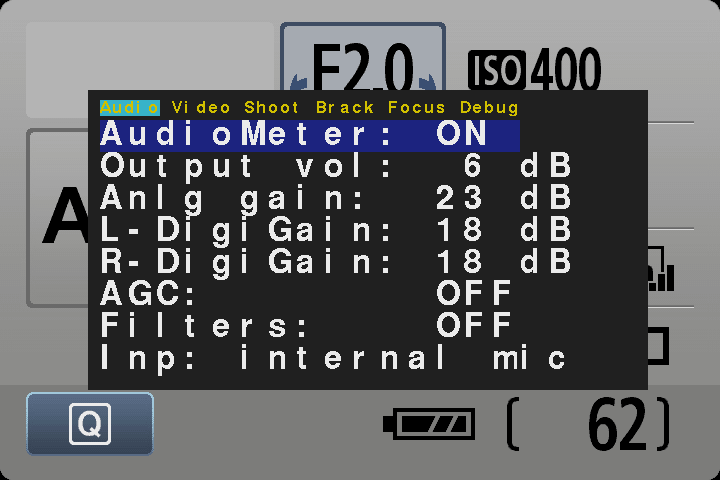
\includegraphics[width=5cm]{AudioMenu-550D.png}}
\end{figure}

\href{http://magiclantern.wikia.com/wiki/Video\%3ARyan\%27s\%20T2i\%20Tips\%20and\%20Reviews\%20-\%20Onboard\%20Mic\%20vs.\%20ATR-3350\%20Lav\%20vs\%20Rode\%20VideoMic}{Video:Ryan's T2i Tips and Reviews - Onboard Mic vs. ATR-3350 Lav vs Rode VideoMic}

Audio tweaks.
\vspace{-10mm}\subsubsection*{}\label{audio-meters}
\textbf{Audio Meters: ON / OFF / MovieOnly}
%
\begin{quote}

Draw the audio meters or not. The \texttt{Movie Only} settings enables audio meters in movie mode only (default).

\end{quote}

\textbf{Output volume (dB)}
%
\begin{quote}

Gain to external audio - currently this is the A/V jack (?) so not audible on just the camera

\end{quote}
\vspace{-10mm}\subsubsection*{}\label{manual-audio-controls}
\textbf{Analog Gain (dB)}
%
\begin{quote}

Gain applied to both inputs in the analog domain - intended as mic-type preamp, but always preferable to digital gain (unless you want different gain or run out of analog).

\end{quote}

\textbf{L-DigitalGain} and \textbf{R-DigitalGain (dB)}
%
\begin{quote}

Digital gain applied separately to the L and R channel.

\end{quote}
\vspace{-10mm}\subsubsection*{}\label{disable-agc}
\textbf{AGC: ON/OFF}
%
\begin{quote}

Enable/disable Automatic Gain Control. Turn this to OFF to prevent hiss noise when recording silence.

\end{quote}

\textbf{Monitor: ON/OFF}
%
\begin{quote}

It's ported from 5D2 code, so it should be tested to see what it does. In the code it says it enables or disables loopback mode (what's this?!)

\end{quote}

\textbf{DigitalFilters: ON/OFF}
%
\begin{quote}

Enable/disable digital audio filters (High Pass Filter, Low Pass Filter and stereo emphasis)

\end{quote}
\vspace{-10mm}\subsubsection*{}\label{input-source}
\textbf{Input}
%
\begin{quote}

Audio input source for recording:
%
\begin{itemize}

\item \textbf{internal mic}

\item \textbf{int Left ext Right}

\item \textbf{external stereo}

\item \textbf{int Left ext Balanced} (internal Left + Right from both external pins as balanced audio)

\item \textbf{Auto int/ext}: camera detects if a mic is plugged in. Int is dual mono, ext is stereo. Does not work with AudioMon builds.

\end{itemize}

\end{quote}
\vspace{-10mm}\subsubsection*{}\label{balanced}\begin{figure}
\noindent\makebox[\textwidth][c]{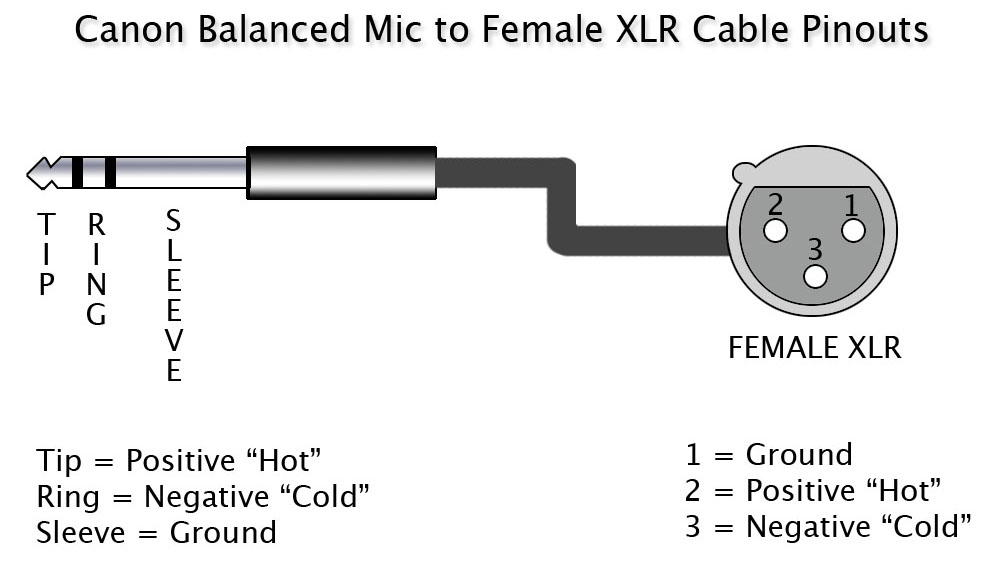
\includegraphics[width=8cm]{XLRtoBalancedCable.jpg}}
\end{figure}

``Balanced audio allows for very long cable runs without interference. Usually balanced mics have three pin XLR connectors and it is very easy to out together an XLR to Canon mic input cable. Balanced allows us to use such pro mics with our little Canons and this is a very welcome surprise for audio guys.'' \href{http://www.cinema5d.com/viewtopic.php?f=39&t=24384&st=0&sk=t&sd=a&start=330\#p164691}{(source)}




%___________________________________________________________________________

\subsection*{LiveV%
  \phantomsection%
  \addcontentsline{toc}{subsection}{LiveV}%
  \label{livev}%
}
\begin{figure}
\noindent\makebox[\textwidth][c]{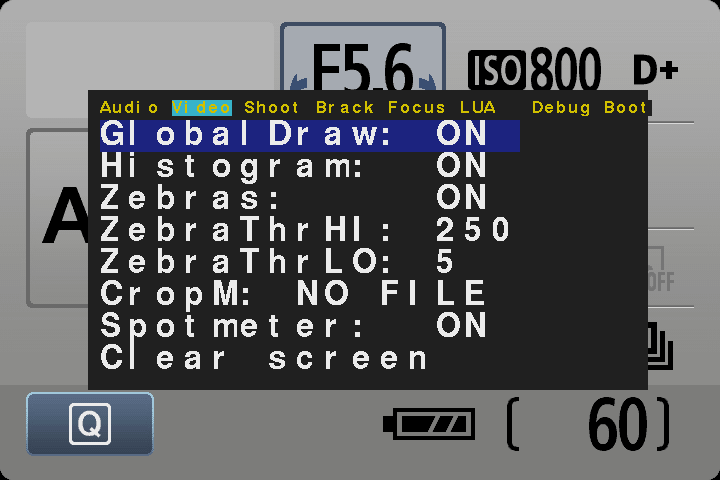
\includegraphics[width=5cm]{VideoMenu-550D.png}}
\end{figure}

LiveView overlays: histogram, zebras, cropmarks, spotmeter, focus peaking, false color...

\textbf{Global Draw: ON/OFF}
%
\begin{quote}

Enable/disable drawing extra graphics elements
(zebra, cropmarks, histogram, waveform, false color, spotmeter, audio meters, ML shooting info...).

Tip: use this to quickly turn them off.

\end{quote}
\vspace{-10mm}\subsubsection*{}\label{histogram}\vspace{-10mm}\subsubsection*{}\label{waveform}
\textbf{Histo/Wavefm: ON/OFF for histogram, OFF/Small/Large for waveform}
%
\begin{quote}

Shows the distribution of image brightness with:
%
\begin{itemize}

\item a histogram plot (toggle with \texttt{SET})

\item a waveform plot (toggle with \texttt{Q})

\end{itemize}

The brightness is considered to be equal to the luma (Y) channel of the LiveView image. Colorspace is YUV.

\end{quote}
\vspace{-10mm}\subsubsection*{}\label{zebras}
\textbf{Zebras: ON/OFF/NRec, lo\_level..hi\_level}
%
\begin{quote}

Enable/disable zebra stripes, which indicate overexposed or underexposed areas.

\texttt{NRec} setting: zebras are only displayed while not recording.

Keys:
%
\begin{itemize}

\item \texttt{SET}: toggle between \texttt{ON/OFF/Auto}

\item \texttt{DISP}: change threshold for underexposure

\item \texttt{Q}: change threshold for overexposure

\end{itemize}

Brightness values are between 0 and 255. A threshold equal to 0 will disable blue zebras, and 255 will disable red zebras.

\end{quote}
\vspace{-10mm}\subsubsection*{}\label{false-color}
\textbf{False color}
%
\begin{quote}

This is an aid for evaluating the exposure. See \href{http://groups.google.com/group/ml-devel/browse_thread/thread/a5db0a709aa86767}{this thread} for details.
%
\begin{itemize}

\item \textbf{Plain C}: full resolution, maybe a bit slow.

\item \textbf{Lo-res C}: half resolution, faster.

\item \textbf{ASM (AJ)}: ASM code by \href{http://magiclantern.wikia.com/wiki/2.0.4_AJ}{AJ}, ported from 5D2. Very fast, but a bit buggy.

\end{itemize}

To get the correct palette, go to LiveView, then Play, make sure you have an image, then back to LiveView.

This function can be triggered by a shortcut key:
%
\begin{itemize}

\item flash button in Movie mode

\item DOF preview button in Photo mode

\end{itemize}

Use \texttt{Q} to enable/disable the shortcut key.

\end{quote}
\vspace{-10mm}\subsubsection*{}\label{cropmark}
\textbf{Cropmks(x/n)}
%
\begin{quote}

Select cropmarks (cycle between them).

There are 3 predefined cropmarks in the zip archive:
%
\begin{itemize}

\item HD with Title \& Action Safe (from CameraRick)

\item Cinemascope

\item Fisheye for stills framing with Samyang/8mm.

\end{itemize}
\begin{figure}
\noindent\makebox[\textwidth][c]{
\includegraphics[width=5cm]{Cropmarks550D.png}}
\end{figure}

If you use custom cropmarks, place them in \texttt{CROPMKS} folder on your SD card and give them short 8.3 names. The number in paranthesis \texttt{Cropmks(x/n)} shows the selected cropmark number and the number of detected cropmarks. You can place at most 9 cropmarks on the card.

An exclamation mark (!) displayed in the menu means there was an error loading the cropmark image.

Get more cropmarks created by Magic Lantern users \href{http://www.sawomedia.de/magiclantern/cropmarks/}{from the ML cropmark repository}.

See \href{http://magiclantern.wikia.com/wiki/Cropmarks}{Cropmarks} for how to create custom cropmarks.

Tip: use \texttt{Debug->Screenshot} to get a bitmap with the correct palette.

Press \texttt{Q} to enable cropmarks in Playback mode.

\end{quote}


\vspace{-10mm}\subsubsection*{}\label{spotmeter}
\textbf{Spotmeter: OFF/Percent/IRE}
%
\begin{quote}

Measure brightness in the center of the frame, and display it as a percentage or IRE value.

Keys:
%
\begin{itemize}

\item \texttt{SET}: change display mode:
%
\begin{itemize}

\item OFF

\item small square $\square$ with text below

\item centered text only

\end{itemize}

\item \texttt{Q}: change measurement unit:
%
\begin{itemize}

\item Percent (0..100\%)

\item IRE -1..101 (formula used by AJ, which maps 0-255 brightness levels to approx. -1..101 IRE)

\item IRE 0..108 (formula proposed by Piers, which maps 16-235 brightness levels to 7.5-100 IRE)

\end{itemize}

\end{itemize}

Note: when using low-contrast picture styles (like Marvels Cine or Superflat), the brightness might not reach the extreme values, even under strong under/over-exposure. This is OK.

\end{quote}
\vspace{-10mm}\subsubsection*{}\label{clean-liveview-display}
\textbf{ClrScreen: OFF/HalfShutter/Always}
%
\begin{quote}

Clear image overlays from LiveView display.
%
\begin{itemize}

\item \textbf{HalfShutter}: Hold the shutter half-pressed, or the \texttt{*} button, or DOF preview for around 1 second,
and this will clear all the overlays from the Live View display (audio, zebra, crops, shutter speeds...).
It allows you to compose the picture without any extra distractions.

This works best when autofocus is assigned to the \texttt{*} button (from Custom Functions, set CFn.9 to 1: \texttt{Shutter/AE lock button} = \texttt{AE lock/AF}).

Tip: also use it for cleaning up unwanted Magic Lantern garbage left on the screen.

\item \textbf{Always}: In this mode, all the overlays are erased from the screen (100\% clean display). Zebras \& friends are still available when you enter the Q menu, and then disappear.

\end{itemize}

\end{quote}
\vspace{-10mm}\subsubsection*{}\label{focus-peaking}
\textbf{Focus Peak: ON/OFF, threshold, color\_mode}
%
\begin{quote}

Experimental focus peaking.

See \href{http://magiclantern.wikia.com/wiki/Focus\%20Assist}{Focus Assist} and \href{http://groups.google.com/group/ml-devel/browse_thread/thread/d29edd39ae8db9ae}{discussion thread}.
%
\begin{itemize}

\item \texttt{SET}: toggle ON/OFF

\item \texttt{Q}: adjust percentile threshold, between 0.1\% and 5\%.

\item \texttt{DISP}: select color mode
%
\begin{quote}
%
\begin{itemize}

\item one of \texttt{R,G,B,C,M,Y} (a single color)

\item \texttt{cc1}: color coding 1 (show edge detection threshold as color, a single color for the entire frame; warmer = higher)

\item \texttt{cc2}: color coding 2 (show edge strength as color for every pixel)

\end{itemize}

\end{quote}

\end{itemize}

Known bugs:
%
\begin{itemize}

\item it's easily fooled by contrast (or lack of it)

\item it may display red markers even if there's nothing in focus

\end{itemize}

Implementation details:
%
\begin{itemize}

\item Only horizontal edges are detected.

\item Only adjacent pixels which fit in an int32 are considered.

\item Threshold method: percentile (0.1\% ... 5\%).

\item Vertical downsampling: always 2

\item Horizontal downsampling: 2 when recording, else 1.

\end{itemize}

\end{quote}
\vspace{-10mm}\subsubsection*{}\label{focus-graph}
\textbf{Focus Graph: ON/OFF}
%
\begin{quote}

Draws a small graph which shows the \emph{amount} of focus in the AF frame (the little rectangle), over the last few seconds. Focus computation is done by Canon's autofocus algorithm.

Since the function which measures the amount of focus is heavily influenced by other factors (like contrast and exposure), ML attempts to normalize the value.

If you are focusing manually, try to position the lens such as you get a local maxima on the focus graph.

\end{quote}
\vspace{-10mm}\subsubsection*{}\label{zoom-in-face-detect-mode}
\textbf{LiveView Zoom: x5 / x10 / :-)}
%
\begin{quote}

Control the zoom feature in LiveView. Change \texttt{x5/x10} settings with \texttt{DISP} and toggle \texttt{:-)} with \texttt{SET}.
%
\begin{itemize}

\item \texttt{x5}: only \texttt{x5} zoom will be available (disables \texttt{x10} zoom)

\item \texttt{x10}: only \texttt{x10} zoom will be available (disables \texttt{x5} zoom)

\item \texttt{x5x10}: both settings available (Canon default)

\item \texttt{:-)} Enable zoom in Face Detection mode

\end{itemize}

\end{quote}


%___________________________________________________________________________

\subsection*{Movie%
  \phantomsection%
  \addcontentsline{toc}{subsection}{Movie}%
  \label{movie}%
}

Functions specific to movie mode.
\vspace{-10mm}\subsubsection*{}\label{qscale}
\textbf{QScale}
%
\begin{quote}

Controls the H.264 QScale parameter, which affects video bitrate.
Lower values mean higher bitrates. OFF disables QScale control.

When QScale is enabled, camera records in VBR mode (variable bitrate).
When QScale is OFF, the bitrate is (more or less) constant (CBR mode).

See \href{http://magiclantern.wikia.com/wiki/Bit\%20rate}{Bit rate} page for details.

Default range is {[}-1 ... -16{]}. This can be changed from config file,
but qscale is restricted to negative values only,
due to limitations in config file parser.

QScale setting is saved, overrides Canon setting, and it does not take effect if you change it during recording. It will take effect at next movie.

\end{quote}
\vspace{-10mm}\subsubsection*{}\label{auto-restart}
\textbf{Movie Restart: ON/OFF}
%
\begin{quote}

While this setting is on, movie recording will restart automatically, unless stopped by you.

\end{quote}
\vspace{-10mm}\subsubsection*{}\label{movie-logging}
\textbf{Movie logging: ON/OFF}
%
\begin{quote}

If this setting is \texttt{ON}, Magic Lantern will write out a metadata file for the each movie to \texttt{MVI\_1234.LOG} (numbered after the movie). The log file contains lens and exposure info, as well as a timestamp every time any of the parameters is changed during recording.

Log files are placed in the same folder as the movies: \texttt{DCIM/100CANON/}, \texttt{101CANON} etc.

Tip: you can rename \texttt{LOG} files to \texttt{CSV} and import them in Excel.

\end{quote}
\vspace{-10mm}\subsubsection*{}\label{custom-af-algorithm}
\textbf{Movie AF: OFF/Hold/Cont}
%
\begin{quote}

Experimental autofocus in movie mode. It overrides the default autofocus algorithm.

Modes:
%
\begin{itemize}

\item \texttt{Hold}: AF only works when you press and hold the shutter halfway, or the \texttt{*} button.
- If you press the Canon AF buton (which is half-shutter or \texttt{*}, depending on your \texttt{CFn.9} setting), the exposure will be changed during autofocus.
- If you press the other button, the exposure will not change during AF, but the AF will be slower.

\item \texttt{Cont}: AF works continuously. It will work faster when you hold the AF button.

\item \texttt{CFPk}: a very experimental version which does not use Canon's focus estimation, but focus peaking data. It only uses the center area and computes the absolute value of edge strengths and divides by the image brightness. Fast in theory, very bad in practice.

\end{itemize}

This is a modified gradient descent algorithm. Tuning parameters (change with \texttt{Q/DISP}):
%
\begin{itemize}

\item \texttt{A=1..64}: aggressiveness (target \% rate of change for focus magnitude).

\item \texttt{N=0..9}: noise filter (for focus derivative).

\end{itemize}

Tips:
%
\begin{itemize}

\item if you see it hunting in the wrong direction, a quick press of half-shutter or \texttt{*} will fix this. If you are holding the AF button pressed, de-press it and press it again to reverse the direction. Be aware that this algorithm has a very high self-esteem and sometimes it will refuse to believe you :)

\item get an external microphone and place it far away from the camera (AF is noisy)

\end{itemize}

\end{quote}

\textbf{Start with LV: ON / Movie mode / All modes}
%
\begin{quote}

Force LiveView on startup. In movie mode, this only has effect if you use unchipped lenses. You can also force LiveView at startup in all modes.

\end{quote}
\vspace{-10mm}\subsubsection*{}\label{change-movie-position}
\textbf{MovieModeRemap: A-DEP / CA}
%
\begin{quote}

Changes movie position on the mode dial. You can swap movie mode with either \texttt{A-DEP} or \texttt{CA}.

\end{quote}
\vspace{-10mm}\subsubsection*{}\label{time-remaining-display}
\textbf{Time Indicator: OFF / Elapsed / Remain.Card / Remain.4GB}
%
\begin{quote}

When recording a movie, ML will display a small time counter in the upper right corner,
which can be:
%
\begin{itemize}

\item \texttt{Elapsed}: duration of the current clip

\item \texttt{Remain.Card}: estimated amount of recording time remaining on the card.

\item \texttt{Remain.4GB}:  estimated amount of recording time until reaching 4GB (or until filling the card, whichever comes first).

\end{itemize}

Unlike Canon's timer which assumes constant bitrate, ML timer assumes variable bitrate and works even if QScale is enabled.
However, due to variations in bitrate, the estimated value will fluctuate a lot, and this is normal.

\end{quote}


%___________________________________________________________________________

\subsection*{Shoot%
  \phantomsection%
  \addcontentsline{toc}{subsection}{Shoot}%
  \label{shoot}%
}
\begin{figure}
\noindent\makebox[\textwidth][c]{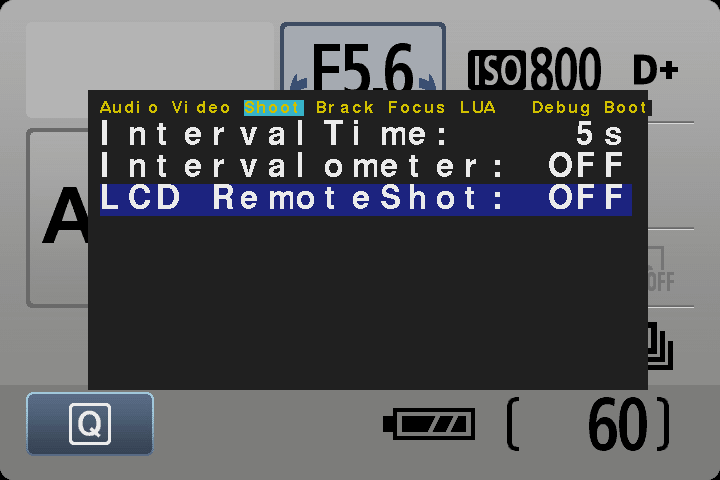
\includegraphics[width=5cm]{ShootMenu-550D.png}}
\end{figure}

Functions for stills shooting.
\vspace{-10mm}\subsubsection*{}\label{exposure-bracketing}
\textbf{HDR Brack}
%
\begin{quote}

AE Bracketing for HDR images and timelapses.

Select number of images with \texttt{SET} and step size with \texttt{DISP}. To turn this off quickly, press \texttt{Q}.

In \texttt{M} mode, this function does shutter bracketing. In the other modes it does exposure compensation bracketing.

HDR images can be taken with:
%
\begin{itemize}

\item ML remote triggers: LCD face sensor \& audio trigger.

\item ML intervalometer (for HDR timelapse)

\item Press the shutter. In this case, the first image will have the middle exposure (without EV compensation), and the 2-second self-timer will be used. Also, this mode only works with 3 images or more.

\end{itemize}

For each HDR picture set, Magic Lantern also writes a bash script for stacking the exposures
with \href{http://wiki.panotools.org/Enfuse}{enfuse}. The scripts are stored in \texttt{DCIM/\#\#\#CANON} and are named after the first picture in set,
e.g. if the HDR sequence is created from \texttt{IMG\_1001.JPG ... IMG\_1005.JPG}, the HDR script will be named
\texttt{HDR\_1001.SH} and the resulting HDR image will be saved as \texttt{HDR\_1001.JPG}.

To run the HDR scripts on the computer, move the scripts and the JPGs in the same directory and run (for example):
%
\begin{quote}{\ttfamily \raggedright \noindent
bash~HDR\_1001.SH
}
\end{quote}

or, for processing all the images at once:
%
\begin{quote}{\ttfamily \raggedright \noindent
for~f~in~\$(ls~*.SH);~do~bash~\$f~;~done
}
\end{quote}

On Windows, you can use Cygwin or MSYS to run the scripts.

Don't forget to delete the scripts from the card; the camera won't delete them!

\end{quote}
\vspace{-10mm}\subsubsection*{}\label{intervalometer}
\textbf{Take a pic every X seconds} / \textbf{Record Y seconds, pause X seconds}
%
\begin{quote}

Change the intervalometer settings (first setting appears in photo mode, second appears in movie mode).

\end{quote}

\textbf{Intervalometer: ON/OFF}
%
\begin{quote}

\href{http://magiclantern.wikia.com/wiki/Video\%3AT2i\%20Timelapse}{Video:T2i Timelapse}

Start/stop intervalometer.
%
\begin{itemize}

\item In photo mode, it takes a sequence of photos with a fixed delay.

\item In movie mode, it takes a sequence of small videos
%
\begin{itemize}

\item When \texttt{HDR Bracket} is active, each movie will be exposed according to the bracketing settings, and the duration of the movie will be multiplied by number of exposures.

\item To use the intervalometer in movie mode, make sure \texttt{Silent Picture} is \texttt{OFF}.

\end{itemize}

\end{itemize}

Tips:
%
\begin{itemize}

\item shoot in manual mode and switch the lens to MF.

\item for power saving, cover the LCD sensor with something.

\item to save the shutter count when doing timelapses, enable \texttt{Silent Picture} or use the intervalometer in Movie mode.

\end{itemize}

\end{quote}
\vspace{-10mm}\subsubsection*{}\label{lcd-face-sensor}
\textbf{LCD Remote Shot: OFF/Near/Away}
%
\begin{quote}

Start/stop remote shutter release mode with the LCD sensor.
%
\begin{itemize}

\item \textbf{Near}: To take a picture, put your hand near the LCD sensor.

\item \textbf{Away}: Picture is taken when you get your hand away from the sensor.

\item \textbf{Wave}: Picture is taken after you wave your hand 3 times near the sensor.

\end{itemize}

This is useful for avoiding camera shake without extra \$\$\$,
especially if you don't have a sturdy tripod.

To use it, select one of P,S,A,M modes, turn OFF Live View,
and make sure ``LCD auto off'' is enabled (in the Canon menu, wrench 1).

\end{quote}
\vspace{-10mm}\subsubsection*{}\label{audio-trigger}
\textbf{Audio RemoteShot: ON/OFF}
%
\begin{quote}

Start/stop remote audio trigger. To take a picture, make some loud noise, for example, clap your hands or pop a balloon.

Audio threshold can be set from \texttt{magic.cfg} by changing \texttt{audio.release.level} (default 700), or by adjusting the audio volume.

You can also start movie recording with this feature.

In photo mode, you can combine this option with the self-timer (may be useful for group or self pictures).

Be careful: this may trigger the shutter from the sounds made by camera (like focus beep or liveview switch).

\end{quote}

You can stop the intervalometer and remote shooting modes either frrom ML menu, or by pressing \texttt{PLAY} or \texttt{MENU}.
\vspace{-10mm}\subsubsection*{}\label{trap-focus}
\textbf{Trap Focus: OFF/Hold/Cont.}
%
\begin{quote}

Takes a picture when the subject comes into focus.

Modes:
%
\begin{itemize}

\item \texttt{Hold}: You hold the shutter half-pressed; camera takes a picture when something comes into focus.

\item \texttt{Cont.}: You don't have to hold the shutter half-pressed; ML will emulate half-shutter presses instead. This will disable some buttons (like \texttt{MENU} and \texttt{PLAY}), so turn it off from ML menu before doing anything else.

\end{itemize}

Trap focus works only when the lens is set to Manual focus (MF).
%
\begin{itemize}

\item Outside LiveView, it only works with lenses with chip.

\item In LiveView it only works for photos, in \texttt{Hold} mode, and it will take a picture
when the focus indicator has (almost) maximum value on the \hyperref[focus-graph]{focus graph}.

Notes:
%
\begin{itemize}

\item You may have to turn the lens back and forth a few times in order to let ML
compute the correct focus scaling for the current scene.

\item If you move from a high-contrast scene to a low-contrast one, you will also have to wait a bit until the high-contrast data disappears from the focus graph.

\end{itemize}

To use Trap Focus in LiveView, make sure \hyperref[focus-graph]{focus graph} is \texttt{ON}.

\end{itemize}

\end{quote}
\vspace{-10mm}\subsubsection*{}\label{flash-no-flash}
\textbf{Flash / No flash: ON/OFF}
%
\begin{quote}

This will toggle flash setting (on/off) after each photo:
%
\begin{itemize}

\item Even pictures (by file number) will be taken without flash

\item Odd pictures will be taken with flash

\end{itemize}

This function works only in P,A,S,M modes. The effect is somewhat similar to Fuji's Natural Light with Flash mode.

Don't forget to pop up the flash :)

\end{quote}
\vspace{-10mm}\subsubsection*{}\label{silent-pictures}\vspace{-10mm}\subsubsection*{}\label{slit-scan-pictures}
\textbf{Silent Picture / Silent Pic HiRes / Slit-scan Pic}
%
\begin{quote}

This can take pictures in LiveView mode without moving the mirror. When enabled, it saves uncompressed YUV422 frames from the LiveView buffer when you press the shutter halfway.
%
\begin{itemize}

\item Make sure you don't have autofocus assigned to half-shutter press (put it on \texttt{*} or turn it off)

\end{itemize}

Modes:
%
\begin{itemize}

\item \texttt{Silent Picture}: simple, low-resolution. Image resolution is usually around 1 or 2 MPix, and depends on the current mode (zoom or not, recording or not, and movie resolution). \href{http://magiclantern.wikia.com/wiki/VRAM/550D\#0x44000080}{Details here}.

\item \texttt{Silent Pic Hi-Res}: emulates high-resolution by taking a matrix of small silent pics, in zoom \texttt{x5} mode. You need to have the camera on a tripod and the scene should be almost stationary (a pic is taken in a few seconds). Useful for timelapse. Only works well with manual focus.

\item \texttt{Slit-scan Pic}: this takes distorted images \href{http://people.rit.edu/andpph/text-slit-scan.html}{like these}. This mode is basically an extreme jello effect which can be used in creative ways.

\end{itemize}

Keys:
%
\begin{itemize}

\item \texttt{SET}: toggle modes (normal or hi-res)

\item \texttt{DISP/Q}: toggle between:
%
\begin{itemize}

\item \texttt{Single/Burst} in normal mode

\item available matrix sizes (which give the image resolutions) in Hi-Res mode.

\item timing (number of clocks to skip after each line) in Slit-scan mode.

\end{itemize}

\end{itemize}

Silent picture setting is applied to intervalometer and remote triggers when used in LiveView mode.

Images are saved in \texttt{DCIM/1xxCANON/}, named after last picture/movie taken without this function.

To convert a 422 image to JPEG on the PC, use \href{https://bitbucket.org/hudson/magic-lantern/downloads/422-jpg-v2.exe}{422-jpg.exe} (Windows and Wine) or \href{https://bitbucket.org/hudson/magic-lantern/src/tip/422-jpg.py}{422-jpg.py} (all platforms, you need to install Python, PIL and numpy). Double-click it, then select a single 422 file, or click Cancel and select a folder with 422 files. You can also use this program in command-line.

TODO:
%
\begin{itemize}

\item avoid that horizontal cut in pictures (vsync doesn't help and there's not enough RAM to buffer an entire image)

\end{itemize}

\end{quote}
\vspace{-10mm}\subsubsection*{}\label{bulb-timer}
\textbf{Bulb Timer: 1s...3600s}
%
\begin{quote}

Very long exposures with Bulb mode and ML timer. Only works with remote triggers and intervalometer. You should select \texttt{M} mode and \texttt{BULB} setting from Canon UI before using this.

Tip: you can cancel the exposure earlier by half-pressing the shutter button.

\end{quote}
\vspace{-10mm}\subsubsection*{}\label{image-settings}

%___________________________________________________________________________

\subsection*{Expo%
  \phantomsection%
  \addcontentsline{toc}{subsection}{Expo}%
  \label{expo}%
}
\begin{figure}
\noindent\makebox[\textwidth][c]{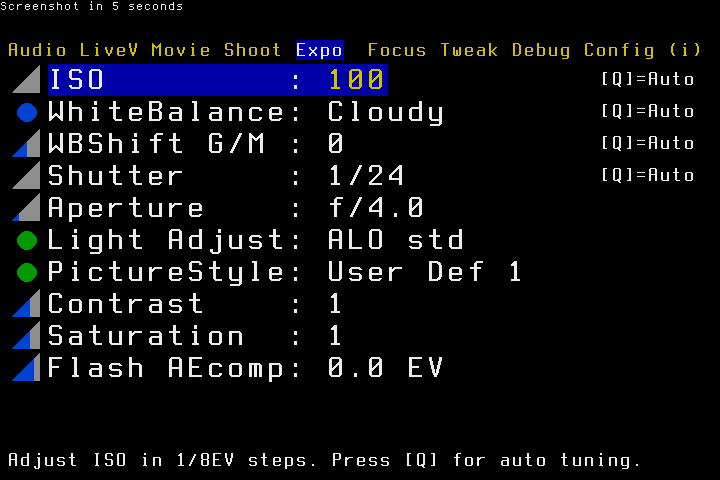
\includegraphics[width=5cm]{ExpoMenu-550D.png}}
\end{figure}

Adjusting the exposure parameters. Most of these settings only work in Manual (photo and video), and some of them work in P, Av and Tv too.
\vspace{-10mm}\subsubsection*{}\label{iso}
\textbf{ISO: 100-25600}
%
\begin{quote}

Custom steps for ISO. Possible values:

0 (Auto), 100, 110, 115, 125, 140, 160, 170, 185, 200, 220, 235, 250, 280, 320, 350, 380, 400, 435, 470, 500, 580, 640, 700, 750, 800, 860, 930, 1000, 1100, 1250, 1400, 1500, 1600, 1750, 1900, 2000, 2250, 2500, 2750, 3000, 3200, 3500, 3750, 4000, 4500, 5000, 5500, 6000, 6400, 7200, 8000, 12800, 25600.

To get ISO values higher than 6400, turn on ISO Expansion from Custom Functions (CFn 1). To get ISO lower than 200, turn HTP off.
In video mode, ISO only goes up to 6400. These is also true without ML.

In manual exposure modes (photo and video), press the \texttt{Q} button on this entry to set the ISO value automatically.
%
\begin{itemize}

\item When LiveView is active, a binary search algorithm is used; the search criteria is a good balance between overexposure and underexposure; search resolution is 1/8EV. If the contrast is very low, the histogram will be centered.

\item When LiveView is off, ISO is set using the Auto ISO feature from Canon firmware, in 1EV steps.

\end{itemize}

\end{quote}
\vspace{-10mm}\subsubsection*{}\label{shutter}
\textbf{Shutter: 1/30...1/4000}
%
\begin{quote}

Custom steps for shutter speed. Possible values:

1/30, 33, 37, 40, 45, 50, 53, 57, 60, 67, 75, 80, 90, 100, 110, 115, 125, 135, 150, 160,
180, 200, 210, 235, 250, 275, 300, 320, 360, 400, 435, 470, 500, 550, 600, 640, 720, 800,
875, 925, 1000, 1100, 1200, 1250, 1400, 1600, 1750, 1900, 2000, 2150, 2300, 2500, 2800, 3200,
3500, 3750, 4000.

In manual exposure modes (photo and video), press the \texttt{Q} button on this entry to set the shutter value automatically.
%
\begin{itemize}

\item When LiveView is active, a binary search algorithm is used; the search criteria is a good balance between overexposure and underexposure; search resolution is 1/8EV. If the contrast is very low, the histogram will be centered.

\item When LiveView is off, the shutter value is computed with the help of Auto ISO feature from Canon firmware, in 1EV steps. This feature is still experimental and sometimes it does not work.

\end{itemize}

\end{quote}
\vspace{-10mm}\subsubsection*{}\label{kelvin-white-balance}
\textbf{WhiteBalance: 1700...10000}
%
\begin{quote}

Kelvin white balance.

In LiveView, press the \texttt{Q} button on this entry to set the WB temperature using the center color as reference gray. The measurement area is 200x200 pixels, centered.

\end{quote}

\textbf{WBShift G/M: G9...0...M9}
%
\begin{quote}

Green-Magenta white balance shift. Useful for fluorescent lighting.

\end{quote}

\textbf{PictureStyle}
%
\begin{quote}

Change picture style. You can see the effect on LiveView instantly.

\end{quote}

\textbf{Contrast/Saturation: -4..4}
%
\begin{quote}

Adjusts the contrast and the saturation of the current picture style.

\texttt{WARNING}: this will modify your current picture style.

\end{quote}

\textbf{Light Adjust: OFF/ALO strong/HTP}
%
\begin{quote}

Select the light adjustment algorithm:
%
\begin{itemize}

\item OFF

\item Auto Lighting Optimizer (strong)

\item Highlight Tone Priority.

\end{itemize}

\end{quote}


%___________________________________________________________________________

\subsection*{Brack%
  \phantomsection%
  \addcontentsline{toc}{subsection}{Brack}%
  \label{brack}%
}

Bracketing was replaced by \texttt{HDR Bracket} feature from the \texttt{Shoot} menu, and it is no longer available. The source code is still there, you can enable it from Makefile and create a custom build.


%___________________________________________________________________________

\subsection*{Focus%
  \phantomsection%
  \addcontentsline{toc}{subsection}{Focus}%
  \label{focus}%
}
\begin{figure}
\noindent\makebox[\textwidth][c]{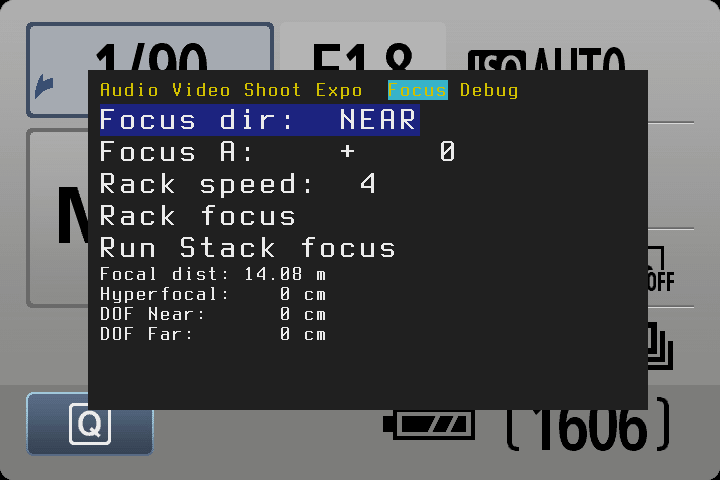
\includegraphics[width=5cm]{FocusMenu-550D.png}}
\end{figure}
\vspace{-10mm}\subsubsection*{}\label{rack-focus}
\href{http://magiclantern.wikia.com/wiki/Video\%3AMagic\%20Lantern\%20for\%20Canon\%20550D\%20-\%20Rack\%20Focus\%20Tutorial}{Video:Magic Lantern for Canon 550D - Rack Focus Tutorial}

\textbf{Focus dir}
%
\begin{quote}

This is the direction the lens moves when pressing the camera's Zoom Out button to set the focus start and end points.

\end{quote}

\textbf{Focus A}
%
\begin{quote}

This is end point of rack focus. To set, focus the lens with the Zoom Out button, then press ``Set''.

\end{quote}

\textbf{Rack Focus}
%
\begin{quote}

Triggers the rack focus operation that moves between the start and end focus points. After the move is complete pressing again reverses the move.

\end{quote}
\vspace{-10mm}\subsubsection*{}\label{focus-stacking}
\textbf{Run Stack focus}
%
\begin{quote}

This selection will shoot a series of photographs with varying focal distances. You can also call this ``focus bracketing''.
It is used in macro photography to assemble sharper final images by merging photos where each has a different focus point.

To configure focus step and number of photos, use the hidden settings \texttt{focus.step} and \texttt{focus.count}.

\end{quote}
\vspace{-10mm}\subsubsection*{}\label{focus-and-dof-info}
The following items are display only:

\textbf{Focal Dist}
%
\begin{quote}

The distance to the focal point. Value is returned by most newer Canon lenses. If the lens does not report any distance information, 0 will be displayed and the DOF calculations will not be correct.

See also \href{http://magiclantern.wikia.com/wiki/Focus\%20distance}{Focus distance}.

\end{quote}

\textbf{Hyperfocal}
%
\begin{quote}

The hyperfocal distance is the point of focus where everything from half that distance to infinity falls within the depth of field. This is the largest depth of field possible for the current f-number.

\end{quote}

\textbf{DOF Near}
%
\begin{quote}

The nearest distance in which objects appear in focus.

\end{quote}

\textbf{DOF Far}
%
\begin{quote}

The farthest distance in which objects appear in focus.

\end{quote}

See also the description from the \href{http://magiclantern.wikia.com/wiki/Magic_Lantern_0.1.6_User_Manual\#Focus_menu}{5D2 ML User Guide}.

\textbf{How rack focus works}

Now that you know what the buttons are about, here is how you make it work:
\newcounter{listcnt0}
\begin{list}{\arabic{listcnt0}.}
{
\usecounter{listcnt0}
\setlength{\rightmargin}{\leftmargin}
}

\item After opening the focus menu, pick the end point of your rack focus, focusing manually with your lens on that point.

\item Next on the Focus Menu, select the direction you will have to focus to in order to find the start point. If the start point is a closer focus, pick \texttt{Near}, if it a farther away focus point, pick \texttt{Far}. ( Remember, you are simply telling camera which direction to go to find the start point.)

\item Next, scroll down to \texttt{Focus A}. You need to zero this setting out, before going on. Press \texttt{Set} to zero it out.

\item Once that is completed you will use the \texttt{Zoom Out} or \texttt{Half Shutter} button to move the focus point to your start point.

\item Next select the time period of the pull, by scrolling down to rack speed. The lower the number, the longer the rack will take. It is recommended for testing purposes to start around 20.

\item Next, start movie recording (you can do that while ML menu is active).

\item Once the camera is recording, scroll to \texttt{Rack Focus}. To start the rack focus, press \texttt{Set}. You should see the rack focus commence and complete its cycle.

\item To return to the beginning point, you can press \texttt{Set} again to return to that point, once again.
\end{list}

\textbf{Note:} the rack focus command may ``stutter'' while racking with some lenses, causing overshoot or undershoot of the desired position. This feature is still under development and should be more mature in a later version.


%___________________________________________________________________________

\subsection*{Debug%
  \phantomsection%
  \addcontentsline{toc}{subsection}{Debug}%
  \label{debug}%
}
\begin{figure}
\noindent\makebox[\textwidth][c]{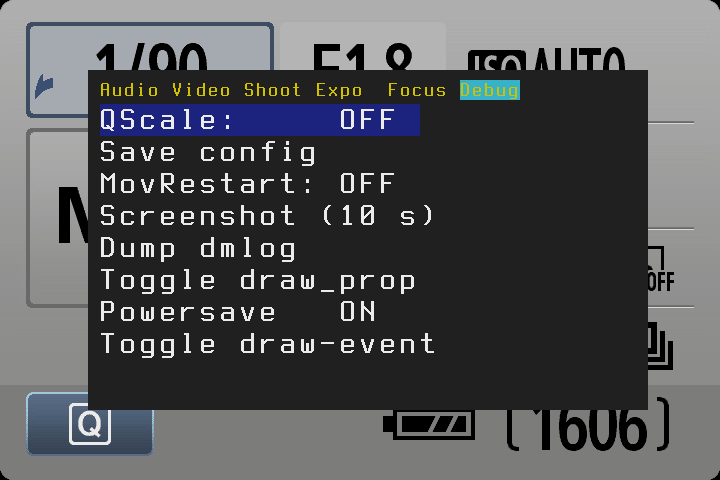
\includegraphics[width=5cm]{DebugMenu-550D.png}}
\end{figure}

\textbf{Save config}
%
\begin{quote}

Save current settings to \texttt{MAGIC.CFG}.

\end{quote}

\textbf{Draw palette}
%
\begin{quote}

Tests the 8-bit bitmap palette, which is used for video overlays. See \href{http://magiclantern.wikia.com/wiki/VRAM}{VRAM}.

\end{quote}

\textbf{Screenshot (10 s)}
%
\begin{quote}

Print screen after 10 seconds (it saves a BMP file).
Only the bitmap overlays are included in the screenshot (i.e. no live view image).

\end{quote}

\textbf{Dump dmlog}
%
\begin{quote}

Saves a log which contains DebugMsg output.
See \href{http://magiclantern.wikia.com/wiki/Debugging\%20Magic\%20Lantern}{Debugging Magic Lantern} page.

\end{quote}

\textbf{Spy prop/evt/mem}
%
\begin{quote}
%
\begin{itemize}

\item prop: display property changes in real-time. See \href{http://magiclantern.wikia.com/wiki/Properties}{Properties}.

\item evt: Display GUI events in real-time. See \href{http://magiclantern.wikia.com/wiki/GUI_Events/550D}{GUI\_Events/550D}.

\item mem: Display memory addresses which change, but not those which change like mad.
Useful for detecting interesting addresses inside the camera RAM (like sensor \& button locations).

Start address and size is selected with the hidden settings (from \texttt{magic.cfg}) \texttt{debug.mem-spy.*}
(see \texttt{debug.c} for details). You can also display only ``small'' or ``boolean'' values.

Trying to spy the camera\_engine addresses seems to cause trouble (camera freeze).
Probably it's not safe to read data from those areas.

\end{itemize}

\end{quote}

\textbf{Powersave}
%
\begin{quote}

Disable the powersave so that the LiveView never shuts off.

WARNING -{}- this can cause problems with your sensor!

\textbf{DO NOT LEAVE THE CAMERA ON CONTINUOUSLY!}

\end{quote}

Some items from this menu may not be available in release builds;
you can uncomment them from \texttt{debug.c} and create a custom \texttt{autoexec.bin}.


%___________________________________________________________________________

\section*{Extra info displays%
  \phantomsection%
  \addcontentsline{toc}{section}{Extra info displays}%
  \label{extra-info-displays}%
}


%___________________________________________________________________________

\subsection*{Main shooting screen (outside LiveView)%
  \phantomsection%
  \addcontentsline{toc}{subsection}{Main shooting screen (outside LiveView)}%
  \label{main-shooting-screen-outside-liveview}%
}
\vspace{-10mm}\subsubsection*{}\label{clock}\begin{figure}
\noindent\makebox[\textwidth][c]{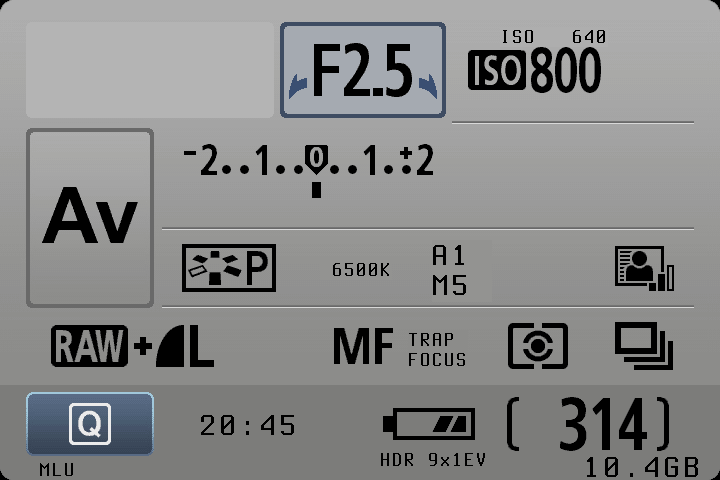
\includegraphics[width=5cm]{InfoDisplayShooting-550D.png}}
\end{figure}
%
\begin{itemize}

\item Clock (bottom of screen)

\item ISO value in finer increments (above Canon's ISO display)

\item Trap Focus status (near MF icon)

\item Kelvin temperature (in the white balance box)

\item WB shift values for BA and GM

\item Flash setting (under clock)

\item HDR setting (under battery icon)

\end{itemize}


%___________________________________________________________________________

\subsection*{MENU->DISP%
  \phantomsection%
  \addcontentsline{toc}{subsection}{MENU->DISP}%
  \label{menu-disp}%
}
\vspace{-10mm}\subsubsection*{}\label{shutter-count}\vspace{-10mm}\subsubsection*{}\label{cmos-temperature}\begin{figure}
\noindent\makebox[\textwidth][c]{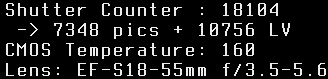
\includegraphics[width=3cm]{InfoMenuDisp-550D.png}}
\end{figure}
%
\begin{itemize}

\item Shutter counter. Only counts pictures taken, not LV switches or quick focus attempts.

\item CMOS temp: temperature of the CMOS sensor (EFIC temperature), in raw units. Before, this was in the Debug menu.

\item Lens name

\end{itemize}


%___________________________________________________________________________

\subsection*{LiveView%
  \phantomsection%
  \addcontentsline{toc}{subsection}{LiveView}%
  \label{liveview}%
}
%
\begin{itemize}

\item Aperture, shutter, ISO

\item Spotmeter: brightness percentage from the center of the frame. Computed as average value of Y component from YUV LiveView buffer over a very small area.

\item Lens focal length and focus distance: see \href{http://magiclantern.wikia.com/wiki/Focus_distance}{Focus\_distance}

\item Exposure compensation (codenamed AE)

\end{itemize}


%___________________________________________________________________________

\section*{Configuration file%
  \phantomsection%
  \addcontentsline{toc}{section}{Configuration file}%
  \label{configuration-file}%
}

The configuration file (\texttt{MAGIC.CFG}) lets you tweak various hidden settings
using a simple text editor (Notepad, gedit, vi...), and is also used
to save Magic Lantern configuration from the GUI menu.


%___________________________________________________________________________

\subsection*{Saving settings%
  \phantomsection%
  \addcontentsline{toc}{subsection}{Saving settings}%
  \label{saving-settings}%
}

From the Magic Lantern menu, choose Debug -> Save config.
Your config file will be overwritten with current Magic Lantern settings.
Comments from the file will be removed!


%___________________________________________________________________________

\subsection*{Hidden settings%
  \phantomsection%
  \addcontentsline{toc}{subsection}{Hidden settings}%
  \label{hidden-settings}%
}

These settings can not be changed from the ML menu, so they are documented here:
%
\begin{quote}{\ttfamily \raggedright \noindent
\#~if~set~to~1,~disable~the~bootdisk~flag.\\
\#~This~does~the~same~thing~as~Debug->Autoboot~menu~item.\\
\#~Only~for~advanced~users!!!\\
magic.disable\_bootdiskf~=~0\\
~\\
\#~Delay~between~clearing~the~overlay~in~Clear~Preview~mode\\
clear.preview.delay~=~500\\
~\\
\#~Stack~focus~step~size~and~frame~count\\
focus.step~=~100\\
focus.count~=~5\\
~\\
\#~Limits~allowed~for~qscale~control.\\
\#~Since~negative~values~are~not~allowed~in~config~file,\\
\#~put~the~absolute~values~here.~Qscale~can~have~only~negative~values.\\
h264.qscale.max.neg~=~1\\
h264.qscale.min.neg~=~16\\
~\\
\#~Threshold~for~audio~trigger\\
audio.release.level~=~700\\
~\\
\#~Delay~between~two~sub-pics~in~hi-res~silent~pic~mode\\
silent.pic.sweepdelay~=~350\\
~\\
\#~Zebra~density:~0,~1~or~2\\
zebra.density~=~2
}
\end{quote}

\end{document}


